
\documentclass[a4paper,12pt,twoside]{report}
\usepackage[left=3cm,right=2cm,top=4cm,bottom=3cm]{geometry}
\usepackage[utf8]{inputenc}
\usepackage[spanish]{babel}
\usepackage{amsthm}
\usepackage{amsmath}
\usepackage{amsfonts}
\usepackage{pgf,tikz}
\usepackage{graphicx}
\usepackage{float}
\usepackage{cite}
\usepackage{enumerate}
\usepackage{courier}
\usepackage{listings}
\usepackage{mathtools}
\usepackage{color}
\usepackage[version=4]{mhchem}

\definecolor{codegreen}{rgb}{0,0.6,0}
\definecolor{codegray}{rgb}{0.5,0.5,0.5}
\definecolor{codepurple}{rgb}{0.58,0,0.82}
\definecolor{backcolour}{rgb}{0.95,0.95,0.92}

\lstdefinestyle{mystyle}{
	backgroundcolor=\color{backcolour},   
	commentstyle=\color{codegreen},
	keywordstyle=\color{magenta},
	numberstyle=\tiny\color{codegray},
	stringstyle=\color{codepurple},
	basicstyle=\footnotesize\ttfamily,
	breakatwhitespace=false,         
	breaklines=true,                 
	captionpos=b,                    
	keepspaces=true,                 
	numbers=left,                    
	numbersep=5pt,                  
	showspaces=false,                
	showstringspaces=false,
	showtabs=false,                  
	tabsize=2
}

\lstset{style=mystyle}
\usepackage{hyperref}
\graphicspath{ {/data/Documentos/Universidad/Fisymat2018/TFM/shh-signal-model/images/} }
\usepackage[toc,page]{appendix}


\usepackage{graphicx}
\usepackage{verbatim}
\usepackage{latexsym}
\usepackage{mathchars}
\usepackage{setspace}


\setlength{\parskip}{\medskipamount}  % a little space before a \par
\setlength{\parindent}{0pt}	      % don't indent first lines of paragraphs

%UHEAD.STY  If this is included after \documentstyle{report}, it adds
% an underlined heading style to the LaTeX report style.
% \pagestyle{uheadings} will put underlined headings at the top
% of each page. The right page headings are the Chapter titles and
% the left page titles are supplied by \def\lefthead{text}.

% Ted Shapin, Dec. 17, 1986

\makeatletter
\def\chapapp2{Capítulo}

\def\appendix{\par
 \setcounter{chapter}{0}
 \setcounter{section}{0}
 \def\chapapp2{Anexo}
 \def\@chapapp{Anexo}
 \def\thechapter{\Alph{chapter}}}

\def\ps@uheadings{\let\@mkboth\markboth
% modifications
\def\@oddhead{\protect\underline{\protect\makebox[\textwidth][l]
		{\sl\rightmark\hfill\rm\thepage}}}
\def\@oddfoot{}
\def\@evenfoot{}
\def\@evenhead{\protect\underline{\protect\makebox[\textwidth][l]
		{\rm\thepage\hfill\sl\leftmark}}}
% end of modifications
\def\chaptermark##1{\markboth {\ifnum \c@secnumdepth >\m@ne
 \chapapp2\ \thechapter. \ \fi ##1}{}}%
\def\sectionmark##1{\markright {\ifnum \c@secnumdepth >\z@
   \thesection. \ \fi ##1}}}
\makeatother



%%From: marcel@cs.caltech.edu (Marcel van der Goot)
%%Newsgroups: comp.text.tex
%%Subject: illegal modification of boxit.sty
%%Date: 28 Feb 92 01:10:02 GMT
%%Organization: California Institute of Technology (CS dept)
%%Nntp-Posting-Host: andromeda.cs.caltech.edu
%%
%%
%%Quite some time ago I posted a file boxit.sty; maybe it made it
%%to some archives, although I don't recall submitting it. It defines
%%	\begin{boxit}
%%	...
%%	\end{boxit}
%%to draw a box around `...', where the `...' can contain other
%%environments (e.g., a verbatim environment). Unfortunately, it had
%%a problem: it did not work if you used it in paragraph mode, i.e., it
%%only worked if there was an empty line in front of \begin{boxit}.
%%Luckily, that is easily corrected.
%%
%%HOWEVER, apparently someone noticed the problem, tried to correct it,
%%and then distributed this modified version. That would be fine with me,
%%except that:
%%1. There was no note in the file about this modification, it only has my
%%   name in it.
%%2. The modification is wrong: now it only works if there is *no* empty
%%   line in front of \begin{boxit}. In my opinion this bug is worse than
%%   the original one.
%%
%%In particular, the author of this modification tried to force an empty
%%line by inserting a `\\' in the definition of \Beginboxit. If you have
%%a version of boxit.sty with a `\\', please delete it. If you have my
%%old version of boxit.sty, please also delete it. Below is an improved
%%version.
%%
%%Thanks to Joe Armstrong for drawing my attention to the bug and to the
%%illegal version.
%%
%%                                          Marcel van der Goot
%% .---------------------------------------------------------------
%% | Blauw de viooltjes,                    marcel@cs.caltech.edu
%% |    Rood zijn de rozen;
%% | Een rijm kan gezet
%% |    Met plaksel en dozen.
%% |


% boxit.sty
% version: 27 Feb 1992
%
% Defines a boxit environment, which draws lines around its contents.
% Usage:
%   \begin{boxit}
%	... (text you want to be boxed, can contain other environments)
%   \end{boxit}
%
% The width of the box is the width of the contents.
% The boxit* environment behaves the same, except that the box will be
% at least as wide as a normal paragraph.
%
% The reason for writing it this way (rather than with the \boxit#1 macro
% from the TeXbook), is that now you can box verbatim text, as in
%   \begin{boxit}
%   \begin{verbatim}
%   this better come out in boxed verbatim mode ...
%   \end{verbatim}
%   \end{boxit}
%
%						Marcel van der Goot
%						marcel@cs.caltech.edu
%

\def\Beginboxit
   {\par
    \vbox\bgroup
	   \hrule
	   \hbox\bgroup
		  \vrule \kern1.2pt %
		  \vbox\bgroup\kern1.2pt
   }

\def\Endboxit{%
			      \kern1.2pt
		       \egroup
		  \kern1.2pt\vrule
		\egroup
	   \hrule
	 \egroup
   }	

\newenvironment{boxit}{\Beginboxit}{\Endboxit}
\newenvironment{boxit*}{\Beginboxit\hbox to\hsize{}}{\Endboxit}

\pagestyle{empty}

\setlength{\parskip}{2ex plus 0.5ex minus 0.2ex}
\setlength{\parindent}{0pt}

\makeatletter  %to avoid error messages generated by "\@". Makes Latex treat "@" like a letter

\linespread{1.2}
\def\submitdate#1{\gdef\@submitdate{#1}}

\def\maketitle{
  \begin{titlepage}{
    %\linespread{1.5}
    
\includegraphics[scale=0.2]{images/ugr.png}

    \Large Universidad de Granada \\
    %\linebreak
    Máster en Física y Matemática \\
    %\linebreak
    Departamento de Matemática Aplicada
    \rm
    \vskip 1in
    \Large \bf \@title
    
  }
  \vskip 0.2in
  \par
  {\Large \@author}
  \vskip 0.1in
  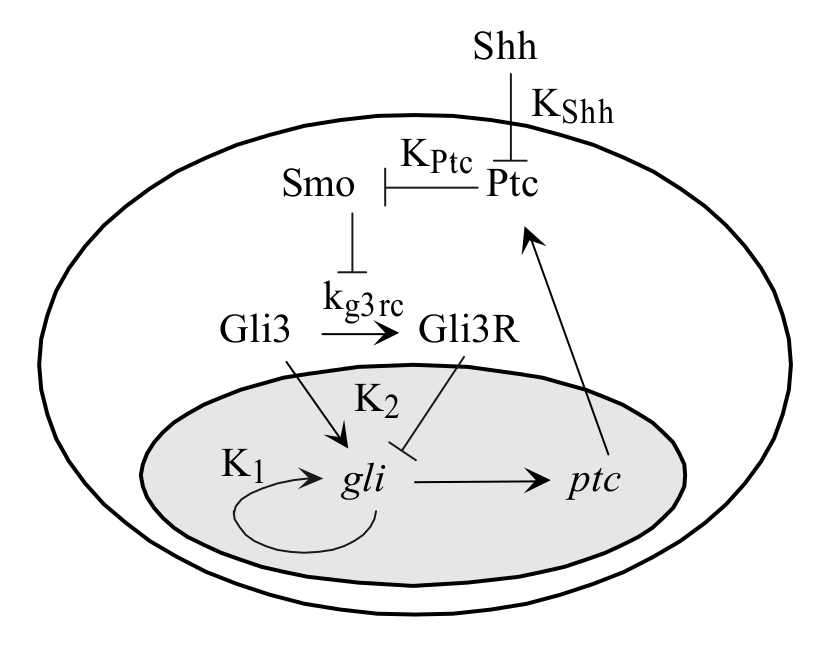
\includegraphics[scale=0.3]{signal_path}
  
 
   \@submitdate
  \vfil
  \end{titlepage}
}

\def\titlepage{
  \newpage
  \centering
  \linespread{1}
  \normalsize
  \vbox to \vsize\bgroup\vbox to 9in\bgroup
}
\def\endtitlepage{
  \par
  \kern 0pt
  \egroup
  \vss
  \egroup
  \cleardoublepage
}

\def\abstract{
  \begin{center}{
    \large\bf Abstract}
  \end{center}
  \small
  %\def\baselinestretch{1.5}
  \linespread{1.5}
  \normalsize
}
\def\endabstract{
  \par
}

\newenvironment{acknowledgements}{
  \cleardoublepage
  \begin{center}{
    \large \bf Agradecimientos}
  \end{center}
  \small
  \linespread{1.5}
  \normalsize
}{\cleardoublepage}
\def\endacknowledgements{
  \par
}

\newenvironment{dedication}{
  \cleardoublepage
  \begin{center}{
    \large \bf Dedication}
  \end{center}
  \small
  \linespread{1.5}
  \normalsize
}{\cleardoublepage}
\def\enddedication{
  \par
}

\def\preface{
    \pagenumbering{roman}
    \pagestyle{plain}
    \doublespacing
}

\def\body{
    \cleardoublepage    
    \pagestyle{uheadings}
    \tableofcontents
    \pagestyle{plain}
    \cleardoublepage
    \pagestyle{uheadings}
    \listoftables
    \pagestyle{plain}
    \cleardoublepage
    \pagestyle{uheadings}
    \listoffigures
    \pagestyle{plain}
    \cleardoublepage
    \pagestyle{uheadings}
    \pagenumbering{arabic}
    \linespread{1.4}
}

\makeatother  %to avoid error messages generated by "\@". Makes Latex treat "@" like a letter


\newcommand{\ipc}{{\sf ipc}}

\newcommand{\Prob}{\bbbp}
\newcommand{\Real}{\bbbr}
\newcommand{\real}{\Real}
\newcommand{\Int}{\bbbz}
\newcommand{\Nat}{\bbbn}

\newcommand{\NN}{{\sf I\kern-0.14emN}}   % Natural numbers
\newcommand{\ZZ}{{\sf Z\kern-0.45emZ}}   % Integers
\newcommand{\QQQ}{{\sf C\kern-0.48emQ}}   % Rational numbers
\newcommand{\RR}{{\sf I\kern-0.14emR}}   % Real numbers
\newcommand{\KK}{{\cal K}}
\newcommand{\OO}{{\cal O}}
\newcommand{\AAA}{{\bf A}}
\newcommand{\HH}{{\bf H}}
\newcommand{\II}{{\bf I}}
\newcommand{\LL}{{\bf L}}
\newcommand{\PP}{{\bf P}}
\newcommand{\PPprime}{{\bf P'}}
\newcommand{\QQ}{{\bf Q}}
\newcommand{\UU}{{\bf U}}
\newcommand{\UUprime}{{\bf U'}}
\newcommand{\zzero}{{\bf 0}}
\newcommand{\ppi}{\mbox{\boldmath $\pi$}}
\newcommand{\aalph}{\mbox{\boldmath $\alpha$}}
\newcommand{\bb}{{\bf b}}
\newcommand{\ee}{{\bf e}}
\newcommand{\mmu}{\mbox{\boldmath $\mu$}}
\newcommand{\vv}{{\bf v}}
\newcommand{\xx}{{\bf x}}
\newcommand{\yy}{{\bf y}}
\newcommand{\zz}{{\bf z}}
\newcommand{\oomeg}{\mbox{\boldmath $\omega$}}
\newcommand{\res}{{\bf res}}
\newcommand{\cchi}{{\mbox{\raisebox{.4ex}{$\chi$}}}}
%\newcommand{\cchi}{{\cal X}}
%\newcommand{\cchi}{\mbox{\Large $\chi$}}

% Logical operators and symbols
\newcommand{\imply}{\Rightarrow}
\newcommand{\bimply}{\Leftrightarrow}
\newcommand{\union}{\cup}
\newcommand{\intersect}{\cap}
\newcommand{\boolor}{\vee}
\newcommand{\booland}{\wedge}
\newcommand{\boolimply}{\imply}
\newcommand{\boolbimply}{\bimply}
\newcommand{\boolnot}{\neg}
\newcommand{\boolsat}{\!\models}
\newcommand{\boolnsat}{\!\not\models}


\newcommand{\op}[1]{\mathrm{#1}}
\newcommand{\s}[1]{\ensuremath{\mathcal #1}}

% Properly styled differentiation and integration operators
\newcommand{\diff}[1]{\mathrm{\frac{d}{d\mathit{#1}}}}
\newcommand{\diffII}[1]{\mathrm{\frac{d^2}{d\mathit{#1}^2}}}
\newcommand{\intg}[4]{\int_{#3}^{#4} #1 \, \mathrm{d}#2}
\newcommand{\intgd}[4]{\int\!\!\!\!\int_{#4} #1 \, \mathrm{d}#2 \, \mathrm{d}#3}

% Large () brackets on different lines of an eqnarray environment
\newcommand{\Leftbrace}[1]{\left(\raisebox{0mm}[#1][#1]{}\right.}
\newcommand{\Rightbrace}[1]{\left.\raisebox{0mm}[#1][#1]{}\right)}

% Funky symobols for footnotes
\newcommand{\symbolfootnote}{\renewcommand{\thefootnote}{\fnsymbol{footnote}}}
% now add \symbolfootnote to the beginning of the document...

\newcommand{\normallinespacing}{\renewcommand{\baselinestretch}{1.2} \normalsize}
\newcommand{\mediumlinespacing}{\renewcommand{\baselinestretch}{1.2} \normalsize}
\newcommand{\narrowlinespacing}{\renewcommand{\baselinestretch}{1.2} \normalsize}
\newcommand{\bump}{\noalign{\vspace*{\doublerulesep}}}
\newcommand{\cell}{\multicolumn{1}{}{}}
\newcommand{\spann}{\mbox{span}}
\newcommand{\diagg}{\mbox{diag}}
\newcommand{\modd}{\mbox{mod}}
\newcommand{\minn}{\mbox{min}}
\newcommand{\andd}{\mbox{and}}
\newcommand{\forr}{\mbox{for}}
\newcommand{\EE}{\mbox{E}}

\newcommand{\deff}{\stackrel{\mathrm{def}}{=}}
\newcommand{\syncc}{~\stackrel{\textstyle \rhd\kern-0.57em\lhd}{\scriptstyle L}~}

\def\coop{\mbox{\large $\rhd\!\!\!\lhd$}}
\newcommand{\sync}[1]{\raisebox{-1.0ex}{$\;\stackrel{\coop}{\scriptscriptstyle
#1}\,$}}

\newtheorem{theorem}{Teorema}[section]
\newtheorem{defi}{{\it Definición}}[chapter]
\newtheorem{corollary}{Corolario}[theorem]
\newtheorem{lemma}[theorem]{Lema}

\newcommand{\Figref}[1]{Figure~\ref{#1}}
\newcommand{\fig}[3]{
 \begin{figure}[!ht]
 \begin{center}
 \scalebox{#3}{\includegraphics{figs/#1.ps}}
 \vspace{-0.1in}
 \caption[ ]{\label{#1} #2}
 \end{center}
 \end{figure}
}

\newcommand{\figtwo}[8]{
 \begin{figure}
 \parbox[b]{#4 \textwidth}{
 \begin{center}
 \scalebox{#3}{\includegraphics{figs/#1.ps}}
 \vspace{-0.1in}
 \caption{\label{#1}#2}
 \end{center}
 }
 \hfill
 \parbox[b]{#8 \textwidth}{
 \begin{center}
 \scalebox{#7}{\includegraphics{figs/#5.ps}}
 \vspace{-0.1in}
 \caption{\label{#5}#6}
 \end{center}
 }
 \end{figure}
}



\begin{document}
	


\title{\LARGE {\bf Nuevo modelo matemático para el sistema de señalización de la proteína Sonic Heddehog (Shh) }\\
 \vspace*{6mm}
}

\author{Bartolomé Ortiz Viso\\Tutor: Óscar Sánchez }
\submitdate{Septiembre 2018}

\narrowlinespacing
\maketitle

\preface

\addcontentsline{toc}{chapter}{Abstract}

\begin{abstract}
	During human development, cells are exposed to a complex network of regulatory signals, which must  be interpreted correctly in order to success doing functions necessary for the organism. Therefore, the transition of signals and cascades of genetic regulation can be understood as mechanisms of information processing that translate extracellular information into intracellular decisions.
	
	The present work aims to show the differences, in terms of a qualitative behavior, that can be found through these complex systems of biological regulation process through different theoretical approaches.
	
	We were particularly interested in the Shh signaling system, among its many roles during development, patterns spinal cord and limb bud tissue differentiation and controls midbrain and ventral forebrain neuronal differentiation. 
	
	There are a few models that has been described in order to understand its behaviour. The most important was developed in \cite{schaffer}. In particular, these mathematicians use the thermodinamic approach to Shh's gene expression mechanish. This approach, in rough outlines, aim to model the gene transcription systems enumerating all the possible states of the promoter and enchancers of gene transcription activation, and then, relating all of them with their theoretically calculate transcriptional activation level. While these steps can be done in multiple ways, they focused their work on the stimulated approach, which links the transcriptional activity to the transcriptional factors (uniquely).
	
	However, some discrepancies has been observed in biological experiments, mainly focused in the existence of an unique stable state, casting aside the biestable swicht behavior shown in the classic model.
	
	 As a result of these state of the art, we thought it would be necessary to offer a new model that update the classic one, but at the same time, we still want to use the BEWARE approach.
	
	 Our main goal has been to develop and study a new model base on the same BEWARE strategy but approaching it by the recruitment perspective, that is, taking into account the fundamental part of the RNAp in this whole biological process and its hability of produce the transcriptional activation. 
	 
	 This work presents a deduction of our new model based on the approach made in \cite{cambon1} and a qualitative study of both models (old and new) through numerical simulations (numerical integration, parameter tunning, bifurcation diagrams, steady states, etc), our discoveries during these and our conclusions about the new and old models. 
	 
	 Specifically, we linked the biestable behaviour of the old model not only to the Shh/$K_{Shh}$ ratio in our cell but with the basal rate of Gli3 (a common trancription factor in this process). We haven't seen that last link in any paper.
	 
	 Furthermore, we found that our new model offers a surprising searched conclusion. Even though the main thermodinamic operator exhibit a highly similar behaviour, our global simulations show a single steady state, no matter how far we alter our parameters. 
	 
	 We hope that these experiments should motivate a deep analytic research of our new model, because our results suggest it could fit the actual biological paradigm, helping us to understand quite a lot about this important topic.5
	 
	 \textsf{Key Words: \emph{Signaling Systems, Sonic Hedgehog, Math Models, Beware models}}

\end{abstract}


\cleardoublepage

\addcontentsline{toc}{chapter}{Agradecimientos}

\begin{acknowledgements}

I would like to express my gratitude to:
\begin{itemize}
	\item My sister and my parents. Thank you for being there every time I need you.
\end{itemize}

\begin{itemize}
 \item My supervisor: Óscar Sánchez .
 \vspace*{3mm}
\end{itemize}

\end{acknowledgements}


\clearpage

\narrowlinespacing

\vspace*{4mm}

`A mathematician, like a painter or a poet, is a maker of patterns. If his patterns are more permanent than
  theirs, it is because they are made with ideas.'\\
\\
\emph{G. H. Hardy}

\normallinespacing


\body
\chapter{Introducción}

\section{ Motivación y objetivos}
\cite{multiple,cambon1,schaffer,saha,bintu2005transcriptional,parker2011cis,meijer2012numerical}

Durante el desarrollo humano, las células están expuestas a una compleja red de señales reguladoras las cuales deben interpretar correctamente para desarrollar las funcionalidades necesarias requeridas por el organismo.Por tanto, se pueden entender la transducción de señales y las cascadas de regulación genética como mecanismos de procesamiento de la información que traducen la información extracelular en decisiones intracelulares.

El presente trabajo pretende mostrar las diferencias en cuanto a comportamiento cualitativo que se pueden encontrar modelando estos complejos sistemas de regulación biológicos mediante distintos acercamientos teóricos. 

En particular, nos centraremos en el estudio del sistema de señalizacion del Sonic Hedgehog (en adelante Shh). 
El Shh es una proteina que conforma uno de los factores de señalización  canónicos, secretados
para regular la función celular y, por tanto, el desarrollo en numerosos sistemas.
\begin{figure}[h]
	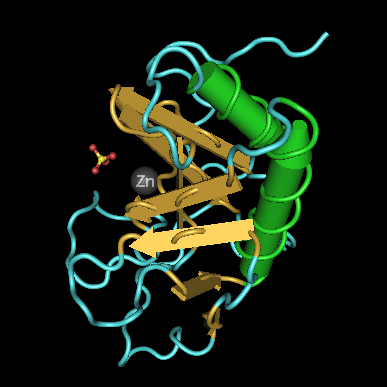
\includegraphics[width=0.5\textwidth]{shh_protein}
	\centering
	\caption{Representación esquemática de la proteina de Shh. Fuente: \cite{wiki:foto_shh}}
\end{figure}


Por ejemplo, la importancia del Shh se pone de manifiesto teniendo en cuenta algunos de sus muchos roles durante el desarrollo: 
\begin{itemize}
	\item Modela la diferenciación del tejido de la médula espinal.
	\item Modela la diferenciación del tejido de la la yema del miembro.
	\item Controla la diferenciación neuronal del mesencéfalo. 
	\item Controla la diferenciación neuronal del prosencéfalo ventral.
\end{itemize}
\small{todo: add references}

Una de las caracteristicas más importantes es que el Shh puede modelar distintos tejidos durante el desarrollo formando un gradiente de concentración. Debido a este gradiente las células detectan su posición dentro del mismo y se diferencian en distintos fenotipos \footnote{Denominamos fenotipo a la expresión del genotipo, es decir, la expresión de los genes, en función de un determinado ambiente.} según la concentración.

Aparte, como se destaca en \cite{schaffer} el Shh también
controla la proliferación de numerosas poblaciones de células durante el desarrollo, incluidas las células granulares del cerebelo. Esto implica que las mutaciones dentro del sistema de señalizacion/regulación del Shh se han asociado con la proliferación de tumores (cáncer) en numerosos tejidos, como en el reciente articulo \cite{clement2007hedgehog}.

Con esta breve introducción ponemos de manifiesto la importancia de conocer el comportamiento de estas redes de señalización. Nuestro interés principal será conocer como afecta de manera cualitativa, un cambio en el procedimiento teorico de modelar los mecanismo bioquimicos involucrados en la expresion genéticas. Centrándonos en redes de regulacion/expresion que relacionan las proteinas\textit{ Ptc, Gli} y \textit{Shh.}

Acotando aún más el sujeto de estudio, los factores de transcripción dentro de la familia \textit{Gli} desempeñan papeles críticos en la mediación e interpretación de las señales de Shh \cite{i1999proteins}. Elucidar cómo funcionan nuestrass redes de regulacion y las proteínas \textit{Gli} nos permitirá ampliar nuestro conocimiento de cómo las células proliferan, diferencian o sobreviven en respuesta a señales de \textit{Shh}, procesos con importancia capital en una gran cantidad de aspectos como por ejemplo \cite{dahmane1997activation}. En especial es importante conocer de qué manera afectan estos cambios a la aparición/desaparición y/o existencia/inexistencia de estados estables. Y, por supuesto, de como están relacionados y como podemos llegar de unos a otros. 
 
 Nuestro trabajo recoge un estudio completo del modelo clásico propuesto en \cite{schaffer}, aportando nueva información dentro del mismo, y un conjunto de experimientos numéricos relacionando nuevos desarrollos teóricos con el modelo clásico. 
 
 Además, al contrario que los artículos originales, todos los códigos se encuentran online y libres para su uso y reproducibilidad, via archivos y via \textit{Jupyter Notebooks}.
 
 Por otra parte, presentamos un estudio teórico y numérico de una nueva forma de modelar desde el enfoque termodinámico este proceso, propuesta en \cite{multiple} para comparar las diferencias cualitativas entre ambos, y avanzar qué posibles resultados podríamos obtener de este nuevo modelo. 
 
 
 \section{Sistema de señalización de Shh}
 
 En esta sección pretendemos ofrecer una visión general de la red de regulación de Shh que se observa en la célula. Todos los modelos usados dentro de este trabajo poseen puntos de vista compartidos, por lo que todas aquellas características que comparten ambos modelos se pueden encontrar aquí.
 
 Asi pues, se puede encontrar en esta sección la descripcion bioquimica del sistema de señalización de Shh y las ecuaciones estándar empleadas en los procesos e interacciones bioquimicas que poseen ambos modelos.
 
 \subsection{Descripción bioquímica del proceso}
 
 La red de señalización de \textit{Shh} comprende la actividad de varias proteínas \ref{figuras} y genes :
 \begin{itemize}
 	\item \textbf{Sonic Hedgehog (Shh)}. Gen: \textit{shh}\footnote{ De forma convencional los genes que codifican una determinada proteína vienen expresados con el mismo nombre, pero en minúscula}
 	\item \textbf{Smothened (Smo}): Receptor de la superficie celular.  
 	\item \textbf{Patched (Ptc)}: Receptor de la superficie celular. Gen: \textit{ptc}
 	\item \textbf{Factores de transcripción \textit{Gli}}:
 	\begin{itemize}
 		\item \textbf{Gli}: Engloba a \textit{Gli1 y Gli2}, puesto que sus funciones son similares. Genes: \textit{gli1, gli2}
 		\item \textbf{Gli3}: Gen: \textit{gli3}
 		\item \textbf{Gli3R}: Resultado de la proteólisis\footnote{La proteólisis es la degradación de proteínas ya sea mediante enzimas específicas, llamadas peptidasas, o por medio de digestión intracelular.} de \textit{Gli3}
 	\end{itemize}
 \end{itemize}
  Además, según la estrategia al modelar, del efecto de la \textbf{\textit{ARN polimerasa}}. 
 
 \begin{figure}[h]
 	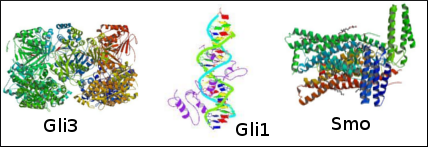
\includegraphics[width=0.8\textwidth]{gli_gli3_smo}
 	\centering
 	\caption{Representación esquemática de la proteinas Gli1, Gli3 y Smo. Fuente: \cite{phosphosite}}
 	\label{figuras}
 \end{figure}
 
 
 
 
 Presentamos el proceso de forma esquemática siguiendo las  indicaciones de \cite{schaffer}:
 \begin{enumerate}
 	\item El \textit{Shh} interactúa con un receptor de superficie celular denominado \textit{Patched }(\textit{Ptc}).
 	\item El \textit{Ptc} inhibe la actividad de señalización de una segunda proteína de la superficie celular: \textit{Smoothened }(\textit{Smo}).
 	\item La unión de \textit{Shh} y \textit{Ptc} neutraliza el efecto inhibidor  de \textit{Ptc} sobre \textit{Smo}.
 	\item Cuando \textit{Smo} no está inhibido afecta a la actividad de la familia de factores de transcripcion \textit{Gli}
 	\item En ausencia de\textit{ Shh, Gli3} es transformado mediante la proteolisis en \textit{Gli3R} (represor de la transcripción génica)
 	\item Tras la señalización de \textit{Shh} y \textit{Smo}, la proteolisis se bloquea, lo que lleva a la acumulación de \textit{Gli3}
 	\item El \textit{Gli3} (activador de la transcripcion génica) activa la transcripcion de los genes \textit{gli1, gli2,ptc, shh.}
 	\item La activación de la transcripción de estos genes provoca la creacion de\textit{ Gli y Ptc}, lo cual a su vez, favorece la generación de \textit{Gli y Ptc}.
 \end{enumerate}
 
 El valor añadido de incluir la ARN polimerasa en el modelo vendrá explicado en la seccion \cite{waseel} .
 En la figura \ref{signal_path} se puede encontrar un dibujo esquemático del proceso.
  \begin{figure}[h]
  	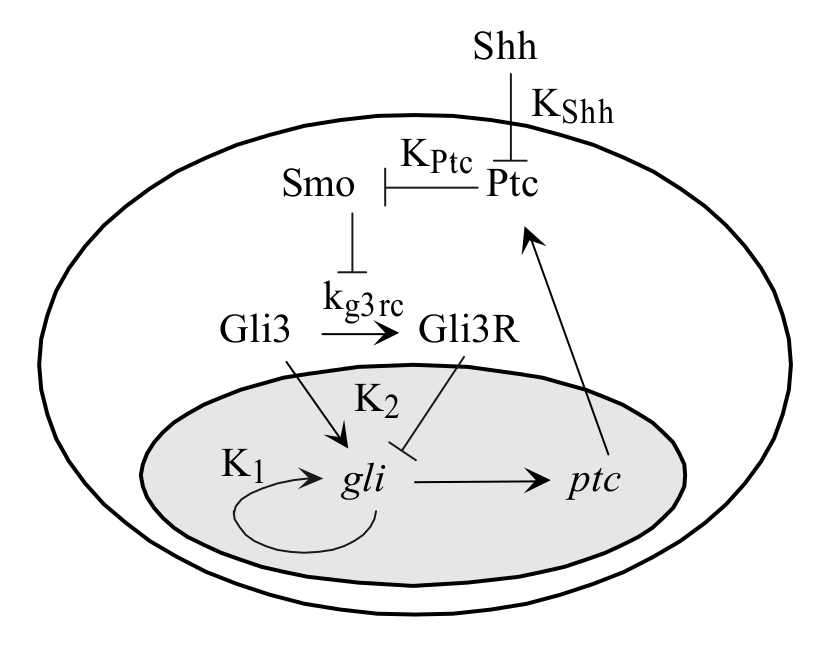
\includegraphics[width=0.8\textwidth]{signal_path}
  	\centering
  	\caption{Representación esquemática de la red de transcripciónn. Fuente: \cite{schaffer}}
  	\label{signal_path}
  \end{figure}
  
 
 
 \subsection{Interacción entre Ptc y Shh}
 Shh y Ptc se unen de forma reversible con una constante de disociación $k_{shh}$ mediante el siguiente esquema: 
 
\begin{equation}
\ce{[Shh] + [Ptc] <->[k_{Shh}] [Shh.Ptc] }
\label{s:1}
\end{equation}
 
 Además, asumimos que las uniones entre Ptc y Shh llegan rapidamente a un estado estacionario si tomamos la escala temporal de transcripcion genetica y sisntesis de proteinas. Para conocer cual es, utilizamos la ecuación de Scatchard.
 
 La ecuación de Scatchard es una ecuación utilizada en bioquímica y biología molecular para calcular la constante de afinidad de un ligando con una proteína, propuesta por primera ver en \cite{scatchard1949attractions}. 
 
 Sea una reaccion como \ref{s:1} tenemos que: 
 $$k_{Shh}=\frac{[Shh.Ptc]}{[Shh][Ptc]}$$
 de donde 
 $$[Shh.Ptc]=k_{Shh}[Shh][Ptc]$$
 Sea ahora $\nu$ representando los moles de ligando unido por mol de proteina, en primer lugar tenemos:
 \begin{equation}
 \nu=\frac{[Shh.Ptc]}{[Ptc_{Total}]}
 \label{s:2}
 \end{equation}
 
 Ahora bien, si operamos:
 $$\nu=\frac{[Shh.Ptc]}{[Ptc_{Total}]}=\frac{[Shh.Ptc]}{[Ptc.Shh]+[Ptc]}=\frac{k_{Shh}[Shh][Ptc]}{[Ptc]+k_{Shh}[Shh][Ptc]}=\frac{K_{Shh}[Shh]}{1+k_{Shh}[Shh]}$$
 Como las constantes de asociacion y disociacion son la misma: \begin{equation}
 \nu=\frac{[Shh]}{[Shh]+K_{Shh}}
 \label{s:3}
 \end{equation}
 
 En este caso, uniendo \ref{s:3} y \ref{s:2} expresión: 
 \begin{equation}
 [Shh.Ptc]=\frac{[Shh][Ptc_{Total}]}{k_{Shh}+[Shh]}
 \label{s:6}
 \end{equation}
 
 \subsection{Señal de transcripcion}
 Vamos a considerar el término \textbf{\textit{Señal}} como la fracción de \textit{Smo} liberada de la inhibicion del \textit{Ptc}. Aunque Ptc y Smo no interactúan fisicamente \cite{schaffer} propone modelarlo de manera similar a la union de Shh y Ptc, puesto que la cantidad de Smo libre puede interpretarse como la cantidad que no esta interactuando de forma eficiente con el Ptc.
 En este caso, tenemos:
 \begin{equation}
 [Shh.Ptc]=\frac{[Ptc_{libre}][Smo_{Total}]}{k_{Ptc}+[Ptc_{libre}]}
 \label{s:5}
 \end{equation}
 Donde $Ptc_{libre}$ hace referencia al Ptc que no está interactuando con Shh y $k_{Ptc}$ es la mitad de la concentración de Ptc necesaria para inhibir la actividad de Smo.
 Tal y como comentamos, definimos la \textbf{\textit{señal}} (en adelante \textit{Signal}) como:
 \begin{equation}
 Signal=\frac{[Smo_{libre}]}{[Smo_{Total}]}=\frac{[Smo_{total}]-[Smo.Ptc]}{[Smo_{Total}]}
 \label{s:4}
 \end{equation}
 Finalmente, usando \ref{s:5} y \ref{s:6} en \ref{s:4} nos queda:
 \begin{equation}
 Signal=\frac{[Smo_{libre}]}{[Smo_{Total}]}=\frac{\frac{Shh}{k_{shh}} + 1}{\frac{Shh}{k_{shh}} + 1 + \frac{Ptc}{k_{ptc}}}
 \label{s:7}
 \end{equation}
 
 \subsection{Dinámica de Gli3 y Gli3R}
 \subsubsection{Dinámica de Gli3}
 En ausencia de señalización Shh, Gli3 se escinde proteolíticamente en un fragmento que funciona como un
 represor transcripcional.En \cite{wang2000hedgehog} muestran que el grado de proteólisis disminuye con el aumento de Shh. En este caso, imponemos que la tasa de proteólisis varíe inversamente con el nivel de señalización Shh en el sistema.
 
 Así, nuestra la cantidad de Gli3 disminuye con una tasa $k_{g3rc}$ que se modifica por la cantidad de $Signal$ en el sistema y un parámetro de saturación $K_g3rc$.
 
 A su vez, se ha demostrado que a medida que se activa la red de regulación génica, gli3 es transcripcionalmente
 reprimido \cite{wang2000hedgehog}. Dos lecturas del grado de activación de nuestra red son Ptc y Gli. 
 
 \textbf{\textit{Esto es importante, puesto que, aunque Ptc ofrece tambien una lectura del grado de activación, los resultados pueden variar en gran cantidad dependiendo de cual elijamos.}}
 
 Por lo tanto, asumimos una relación inversa entre la transcripcion de gli3 y la concentración de Gli en las ecuaciones para Gli3, partiendo de una tasa basal de generacion de Gli3 que viene dada por la constante $r_{g3b}$. 
 
 Finalmente, con toda la información podemos entender como modelar matemáticamente la evolución de Gli3:
 
  \begin{equation}
  \frac{dGli_3}{dt} = \frac{r_{g3b}}{Gli}-k_{deg}Gli_3-\left(\frac{k_{g3rc}}{K_{g3rc}+Signal}\right)Gli_3,
  \end{equation}
 
 \subsubsection{Dinámica de Gli3R}
 La existencia de esta molecula es completamente dependiente a la existencia de Gli3.
 
 En su dinámica vamos a encontrar un término positivo exactamente igual a la rapidez en la que Gli3 es separado de forma proteolitica y, además, un término de degradacion (cuya constate de degradación es igual a la constante de degradación de Gli3).
 
  Esto nos deja con la expresión:

 
 \begin{equation}
 \frac{dGli3R}{dt}= \left(\frac{k_{g3rc}}{K_{g3rc}+Signal}\right)Gli_3-k_{deg}Gli3R,
 \end{equation}
 
 \section{Modelado BEWARE}
\cite{ay2011mathematical}
 \cite{bintu2005transcriptional} \cite{bintu2005transcriptional2}
 \cite{fakhouri2010deciphering}
 \cite{he2010thermodynamics}
 \cite{segal2008predicting}
 \textbf{Rellenar los huecos con estas referencias}
 
 \subsubsection{Enfoques en el modelado de la regulación génica}
 
 El análisis detallado de las redes transcripcionales es clave para comprender los procesos biológicos centrales. Modelar correctamente la regulación de genes es fundamental para tal fin, puesto que la expresión génica está en el nexo de muchos procesos biológicos, y los cambios en los niveles de proteínas reguladoras o enlaces pueden ser la base de, por ejemplo, enfermedades de gran impacto como el cáncer. 
 
  A la hora de profundizar y aportar nuevo conocimiento en este área,las matemáticas se han desarrollado por diversos caminos, resaltando unas u otras características. Como se destaca en \cite{ay2011mathematical} dentro de este actual abanico de técnicas tenemos dos grandes estrategias iniciales: \textit{Enfoque analítico o estadístico}. 
  
  Durante nuestro trabajo nos hemos centrado en el primero. Dentro del cual podemos encontrar tres grandes ramas: \textit{modelos termodinámicos, booleanos y de ecuaciones diferenciales}. Cada una de los cuales debe ser tomada con cautela para obtener el máximo beneficio en cuanto al conocimiento del comportamiento cualitativo y cuantitativo de las soluciones. 
 
 Lo más habitual presentado en el grado y en el máster son los modelos basados en ecuaciones diferenciales, ya sean ordinarias o en derivadas parciales. Estos modelos surgen de la necesidad de crear sistemas dinamicos con muchas componentes que evoluciones a lo largo del tiempo. Como hemos visto en la sección anterior, esta técnica ha sido empleada por los dos modelos estudiados, en aquellos comportamientos dependientes de proteinas que modelaban la asociación y disociación de compuestos.
 
 Sin embargo, a la hora de modelar el proceso de transcripción génetica, tanto para \textit{Gli} como para \textit{Ptc}, el modelado va a seguir \textbf{el enfoque termodinámico}. 
 
 Este enfoque de modelado, como apunta \cite{ay2011mathematical}, busca extraer información sobre la regulación génica a partir de las secuencias de las regiones reguladoras y la unión medida o inferida de los factores de transcripción específicos.
 
 Es decir, supongamos que tenemos un promotor y algunos factores de transcripción que reprimen o promueven esta transcripción. En este caso, nuestro modelado quiere predecir cómo se activará o reprimirá la transcripccion de un gen según estos factores y sus cantidades.
 
 
 La clave fundamental modelando termodinamicamente es el calculo de cómo las diferentes combinaciones de distintos lugares y numeros de union en una región reguladora funcionan juntos para producir la expresión a lo largo del tiempo de un gen.
 
 A grandes rasgos suponemos que la actividad del gen es proporcional al nivel de activadores unidos e inversamente proporcional al nivel de represores.
 
 \subsubsection{Procedimiento}
 
  Sea cual sea la estrategia a seguir, modelado termodinámico sigue dos pasos comunes a todos los modelos de esta rama:
  \begin{itemize}
  	\item En primer luga,: se enumeran todos los estados posibles del potenciador, en función de las posibles interacciones entre el factor de transcripción y el ADN, con un peso estadístico asignado a cada estado.
  	\item  El segundo lugar calculamos el resultado de la expresión génica de cada estado. Los estados con alta ocupación de activadores son más proclives a inducir una expresión alta, mientras que la ocupación del represor puede dar como resultado una baja expresión.
  \end{itemize}
  
   Durante el primer paso es indispensable el calculo de la probabilidad de que un gen se ponga en funcionamiento, para ello calculamos la fracción de los estados con una cantidad de activadores unidos destacable frente a represores.
   
   Esto por si solo ya genera una gran cantidad de estados a tener en cuenta, pensemos en nuestro caso: nuestra región regulatoria tiene tres lugares de unión, por tanto habrá nueve estados posibles, vinculados y no vinculados. Si queremos añadir nueva información (por ejemplo si nos interesamos por elementos con ccinco lugares de unión) el numero de estados aumenta considerablemente (en nuestro caso hipotetico 25 entre vinculados y no vinculados).
 
 
 Otro de los factores a tener en cuenta es el calculo del peso estadístico para un estado. Para ello usamos la concentración de factores de transcripción
 y la afinidad de estos factores por sus sitios en el ADN. Para una unión abundante de proteínas a sitios de alta afinidad, el peso será mucho mayor que en los casos en que la transcripción el factor es escaso o el sitio de unión es débil.
  La probabilidad de cada estado se puede calcular por
 dividiendo el peso estadístico del estado por la suma del peso estadístico de todos los posibles
 estados. 
 
 
 Este proceso de cálculo puede incorporar propiedades que afectan la transcripción. por ejemplo, interacciones cooperativas y competitivas entre factores de transcripción y los efectos inhibidores de los represores sobre los activadores se pueden agregar explícitamente al modelo asignando pesos más altos o más bajos.
 
 Como podemos observar, estamos ante una forma de modelado que nos da bastante juego a la hora de modificar distintos parametros y procedimientos. En particular, vamos a resaltar la mayor diferencia entre los distintos modelados que se han empleado en este trabajo:
 \begin{itemize}
 	\item \cite{schaffer} modela la expresion genica como cantidad proporcional a la suma ponderada de los factores de transcripción.
 	\item Por otra parte, \cite{cambon1} proponen que la expresión génica sea proporcional a la probabilidad de union del ARN-polimerasa (\textit{ enfoque recruitment}), la cual viene modificada por los factores de transcripcion.
 		
 		
 	\end{itemize}
 discutido a continuación, uno puede modelar la producción de expresión génica como proporcional a la unión
 probabilidad de la ARN polimerasa o suma ponderada de los factores de transcripción (
 
 
 
 
 \subsubsection{Críticas recibidas}
 
 
 Finalmente, como último apunte, aunque partimos un de una forma de modelado con amplios resultados queremos resaltar algunas de las criticas que ha recibido esta forma de modelar.
 
 La implementación actual ignora procesos adicionales como la estructura y modificación de la cromatina, o la metilación del ADN, y no trata de forma independiente el reclutamiento de cofactores o la maquinaria general de transcripción.
 
  Se supone que estos saltos teoricos no aportan gran información al sistema. (añadir referencias de esto a parte de \cite{ay2011mathematical})

\chapter{Modelo clásico}

\label{ch:modelo_clasico}

\section{Introducción}
El modelo que planteamos en esta sección pertenece a el modelado considerado clásico realizado en \cite{schaffer}.

Como tenemos gran parte de la dinámica ya planteada, en esta sección, tal y como avanzamos al principio, vamos a presentar la forma en la que se modela la generación de Gli y Ptc (la transcripción génetica) aplicando un enfoque de métodos de termodinámica estadística.

\section{Modelado BEWARE}
 
 
 
 Partimos de dos resultados experimentales que muestran que gli1, gli2 y ptc están regulados transcripcionalmente por la señalización de Shh.
 
  Definimos $K_1$ como la constante de enlace de disociación de equilibrio de Gli y $K_2$ como la constante de enlace de disociación de equilibrio de Gli3 (tanto activador como represor, Gli3R). Las zonas de unión al ADN de todas las formas de Gli están altamente relacionadas, lo que sugiere que estas las afinidades son similares.
  
  Ante la decisión de que cantidad de enlaces tomar, \cite{schaffer}, para simplificar, suponen que hay el mismo número de posibles enlaces Gli dentro de los
  promotores para Gli y Ptc.
  
  
  El promotor puede existir en numerosos
  estados posibles (promotor vacío, dos Gli  y un Gli3 y el resto de combinaciones de 3 elementos). Ademas la probabilidad de cada estado de unión está determinada por las concentraciones relativas de las tres especies (Gli,Gli3, Gli3R) y sus afinidades de unión al ADN. 
  
  
  Nuestro objetivo es desarrollar el modelo de acuerdo a procedimiento BEWARE, por tanto, para modelar el nivel de activación transcripcional del promotor, calculamos la suma de la probabilidad de cada posible estado del promotor multiplicado por una tasa de la activación de transcripción génica que la combinación particular
  induce.
  Sin embargo, para ello debemos determinar correctamente  el nivel de activación para un estado dado, con este fin \cite{schaffer,saha} aplican varias reglas:
  En primer lugar la unión del número máximo de activadores transcripcionales (una combinación de Gli y Gli3) produce un estado con la máxima tasa transcripcional  posible, igual a $(v_{max,G} + r_{bas})$ para el promotor gli.
  
  En este caso $v_{max}$ es la tasa de transcripción inducida máxima y $r_{bas}$ es igual a la tasa basal de transcripción que se obtendría para un promotor completamente independiente.
   Implícita en esta expresión está la suposición de que \cite{schaffer} no tiene en cuenta la dinámica del ARNm, es decir, suponen que cada molécula de ARNm produce un número fijo de proteínas. 
   
   
  A continuación, se permite la posibilidad de unión cooperativa de proteínas al promotor, de forma que el promotor con uno o más factores unidos tuviera una afinidad incrementada para el siguiente factor. A este factor lo denominamos \textit{factor de cooperatividad de unión}$=c$ que habitualmente viene igualado a la unidad ($c=1$).
  
   Además, para cada número de activadores unidos, menores que el número máximo de uniones posibles, la velocidad inducida $v_{max, G}$ se multiplica por un factor $e<1$, para poner de manifiesto de una activación transcripcional menor que la máxima. 

Finalmente, para cada represor transcripcional $Gli3R$ unido, la suma $(v_{max, G}+ r_{bas})$ se multiplica por el factor de represión $r<1$.
  
Con ambos elementos, multiplicamos la probabilidad de cada estado por la tasa de transcripción de cada estado, sumando los elementos resultantes entre sí y simplificando con ayuda de \cite{sympy}. 
 
 El resultado son dos expresiones relativas al proceso promotor y el proceso de transcripción basal:

 \begin{equation}
  Promoter=\frac{\left(Gli K_{2} + Gli_{3} K_{1}\right) \left(3 K_{1}^{2} K_{2}^{2} e^{2} + 3 K_{1} K_{2} c e \left(Gli K_{2} + Gli_{3} K_{1} + 2 Gli3R K_{1} e r\right) + c^{2} \left(Gli^{2} K_{2}^{2} + 3 Gli Gli3R K_{1} K_{2} e r + Gli_{3}^{2} K_{1}^{2} + Gli_{3} K_{1} \left(2 Gli K_{2} + 3 Gli3R K_{1} e r\right) + 3 Gli3R^{2} K_{1}^{2} e^{2} r^{2}\right)\right)}{K_{1}^{2} K_{2}^{2} \left(3 Gli_{3} K_{1} + 3 Gli3R K_{1} + K_{2} \left(3 Gli + K_{1}\right)\right) + 3 K_{1} K_{2} c \left(Gli K_{2} + Gli_{3} K_{1} + Gli3R K_{1}\right)^{2} + c^{2} \left(Gli K_{2} + Gli_{3} K_{1} + Gli3R K_{1}\right)^{3}}
 \label{promoter_1}
 \end{equation}

 \normalsize
 
 
 \begin{equation}
 Basal=\frac{K_{1}^{2} K_{2}^{2} \left(3 Gli K_{2} + 3 Gli_{3} K_{1} + K_{1} \left(3 Gli3R r + K_{2}\right)\right) + 3 K_{1} K_{2} c \left(Gli K_{2} + Gli_{3} K_{1} + Gli3R K_{1} r\right)^{2} + c^{2} \left(Gli K_{2} + Gli_{3} K_{1} + Gli3R K_{1} r\right)^{3}}{K_{1}^{2} K_{2}^{2} \left(3 Gli_{3} K_{1} + 3 Gli3R K_{1} + K_{2} \left(3 Gli + K_{1}\right)\right) + 3 K_{1} K_{2} c \left(Gli K_{2} + Gli_{3} K_{1} + Gli3R K_{1}\right)^{2} + c^{2} \left(Gli K_{2} + Gli_{3} K_{1} + Gli3R K_{1}\right)^{3}}
 \label{basa_1}
 \end{equation}
 
   
\section{Sistema final}
 Con los operadores BEWARE finalmente calculados podemos ya disponer de el sistema dinámico final que modeliza el sistema de señalización de Shh:
 
 \begin{equation}
 \frac{dGli}{dt} = v_{max,G}Promoter+r_{bas,G}Basal-k_{deg}Gli,
 \label{eq1:1}
 \end{equation}
 
 \begin{equation}
 \frac{dGli_3}{dt} = \frac{r_{g3b}}{Ptc}-Gli_3\left(k_{deg}+\frac{k_{g3rc}}{K_{g3rc}+Signal}\right),
 \label{eq1:2}
 \end{equation}
 
 \begin{equation}
 \frac{dGli3R}{dt}= Gli_3\left(\frac{k_{g3rc}}{K_{g3rc}+Signal}\right)-k_{deg}Gli3R,
 \label{eq1:3}
 \end{equation}
 
 \begin{equation}
 \frac{dPtc}{dt} = v_{max,P}Promoter+r_{bas,P}Basal-k_{degp}Ptc.
 \label{eq1:4}
 \end{equation}
 
\section{Estados estacionarios}\label{apartado2.4}
Siguiendo con el estudio estandar que se lleva a cabo en los modelos matemáticos procedemos con un estudio sobre los estados estacionarios que podemos encontrar en nuestro modelo. En primer lugar procedemos afrontando el problema desde una perspectiva analítica. 

Sean las ecuaciones (\ref{eq1:1})(\ref{eq1:2})(\ref{eq1:3})(\ref{eq1:4}), si suponemos que éstas se encuentran en un estado estacionario entonces las concentraciones de las sustancias son constantes. Esto implica que su derivada temporal es igual a cero.

Dado que las ecuaciones continen términos complejos, nos interesamos por agruparlas, de manera que los cálculos no sean más sencillo en un primer intento de extraer información:

Por un lado de (\ref{eq1:1}) y (\ref{eq1:4}):

$$\begin{cases} 0 = v_{max,G}Promoter+r_{bas,G}Basal-k_{deg}Gli, \\0= v_{max,P}Promoter+r_{bas,P}Basal-k_{degp}Ptc. \end{cases}$$
Teniendo en cuenta:

$$
r_{bas,G}=\frac{v_{max,G}}{100},r_{bas,P}=\frac{v_{max,P}}{100}
$$

Si igualamos ambas ecuaciones nos queda:
\begin{equation*}
\frac{k_{deg}}{v_{max,G}}Gli=Promoter+\frac{1}{100}Basal=\frac{k_{degp}}{v_{max,P}}Ptc \implies \frac{v_{max,P}k_{deg}}{v_{max,G}k_{degp}}Gli=Ptc
\end{equation*}

 En particular si llamamos $k_{cc}=\frac{v_{max,P}k_{deg}}{v_{max,G}k_{degp}}$:
 \begin{equation}
k_{cc}Gli=Ptc
\label{gli-ptc}
 \end{equation}


Por otra parte, de (\ref{eq1:2}) y (\ref{eq1:3}):



$$\begin{cases} 0 = \frac{r_{g3b}}{Gli}-Gli_3\left(k_{deg}+\frac{k_{g3rc}}{K_{g3rc}+Signal}\right), \\0=Gli_3\left(\frac{k_{g3rc}}{K_{g3rc}+Signal}\right)-k_{deg}Gli3R. \end{cases}$$

Sumando, obtenemos:

\begin{equation}
\begin{split}
0=\frac{r_{g3b}}{Gli}-Gli_3k_{deg}-k_{deg}Gli3R & \implies \frac{r_{g3b}}{Gli}=Gli_3k_{deg}+k_{deg}Gli3R\implies
\\
& \implies \frac{r_{g3b}}{Gli_3k_{deg}+k_{deg}Gli3R}=Gli
\end{split}
\label{gli3gli}
\end{equation}

Con estas cuentas, podemos obtener, en primer lugar, una función de $Signal$ (\ref{S:7}) modificada gracias a (\ref{gli-ptc}), la llamaremos $Signal_{modificada}$:
\begin{equation}
Signal_{modificada}=\frac{\frac{Shh}{k_{shh}} + 1}{\frac{Shh}{k_{shh}} + 1 + \frac{k_{cc}}{k_{ptc}Gli}}.
\end{equation}

Ahora, sustituimos los valores que tenemos de manera que podamos expresar todas las concentraciones en función de Gli. 

Nuestro objetivo es intentar hallar los estados estacionarios mediante los puntos fijos entre dos expresiones de Gli. Con ello, usando (\ref{gli3gli}) nos quedaría:

\begin{equation}
 \frac{r_{g3b}}{Gli}=Gli_3k_{deg}+k_{deg}Gli3R
 \implies Gli_3=\frac{r_{g3b}(K_{g3rc}+Signal_{modificada})}{k_{deg}(K_{g3rc}+Signal_{modificada})Gli}
\label{equgli3}
\end{equation}
 Y de nuevo, por  (\ref{gli3gli}):
 
 \begin{equation}
 Gli3R=\frac{r_{g3b}}{k_{deg}Gli}-Gli_3
 \label{equgli3r}
 \end{equation}

Debido a la capacidad de expresar Gli3R y $Gli_3$ con respecto a Gli, podemos obtener la variación de Promoter y Basal directamente con Gli, substituyendo en ellos el valor de Gli3R y $Gli_3$
Con ello, finalmente obtenemos una igualdad cuyos puntos fijos nos darán los posibles estados estacionarios. De \ref{eq1:1} igualado a cero :

 \begin{equation}
 Gli=\frac{v_{max,G}}{k_{deg}}Promoter_{modificado}(Gli)+\frac{1}{100}Basal_{modificado}(Gli)
 \label{final_gli}
 \end{equation}


\section{Simulaciones}

En esta sección vamos a desarrollar todas las simulaciones numéricas llevadas a cabo en el estudio cualitativo del modelo de \cite{schaffer}.
Para estudiar este modelo y reproducir algunos resultados, seguimos el siguiente esquema:
\begin{itemize}
	\item \textbf{Recolección y contraste de los parámetros} usados
	\item \textbf{Estudio y comparación de la variabilidad del operador BEWARE}. Dentro de este apartado comparamos numéricamente las reducciones desarrolladas en \cite{multiple} con el fin de asegurar la exactitud de las mismas y, finalmente, usar la forma reducida para obtener programas más eficientes.
	\item \textbf{Análisis numérico de las soluciones estacionarias}: Desarrollamos la formula analítica para obtener un código que nos permita rastrear cambios en el comportamiento cualitativo ante grandes variaciones en los parámetros.
	\item En aquellos parámetros con especial interés por la reproducibilidad o la novedad en su estudio, \textbf{computamos un diagrama de bifurcación}.
\end{itemize}
\subsection{Parámetros}
A menos que se especifique lo contrario, para las simulaciones hemos tomado como valores de parametros los expuesto en la tabla \ref{tabla11}.
\begin{table}[h]
	\begin{center}
		
		\begin{tabular}{ |p{3cm}||c|p{3cm}|p{3cm}|  }
			\hline
			\multicolumn{4}{|c|}{Tabla de parámetros de \cite{schaffer}  } \\
			\hline
			Parámetro & Valor & Descripción & Fuente\\
			\hline
			$Shh $  & $0-30$    &\tiny{Cantidad de Shh} &   \cite{cambon1}\\
			$k_{Shh}$ &  $ 0.58-2.0nM$  & \tiny{Constante de disociación de los enlaces Ptc-Shh}   & \cite{cambon1}\\
			$k_{Ptc} $ & $8.3\times10^{-11}M$ & \tiny{ Mitad de la máxima concentración de Ptc que inhibe la señal de Smo } &  \cite{cambon1}\\
			$k_{deg}$   &$0.009min^{-1} $ & \tiny{ Constante de degradacion de todas las moleculas Gli } &  \cite{cambon1}\\
			
			$k_{g3rc}$ &  $0.012min^{-1}$  & \tiny{ Constante deconversion de Gli3 en Gli3R} & \cite{schaffer}\\
			$r_{g3b}$ & $1.6\times10^{-19}M^2/min$  & \tiny{ Tasa basal de sintesis de Gli3 }   & \cite{schaffer}\\
			$K_{g3rc}$ & $0.1$ & \tiny{ Constante de sensibilidad de la conversioon a fuerza de la señal }   & \cite{schaffer}\\
			
			$k_{deg_p}$& $0.09min^{-1} $ &  \tiny{constante de degradacion de Ptc} & \cite{cambon1}\\
			
			\hline
		\end{tabular}
		
	\end{center}
	\caption{Tabla de parámetros de \cite{schaffer} }\label{param_2}
	\label{tabla11}
\end{table}

\subsection{Variación del operador BEWARE (promoter y basal)}
En primer lugar antes de comenzar la simulación completa comprobamos la reproducibilidad de los operadores que conforma el modelado BEWARE. 

Además, pretendíamos tener una base para comparar posteriormente estos comportamientos con el nuevo operador.

Dentro las figuras se puede apreciar una línea discontinua. Esta línea marca el comportamiento asintótico del nuevo operador BEWARE a modo de adelanto de la siguiente sección. 
Para repetir las simulaciones hemos simulado la variación de Promoter \ref{varipro} y Basal \ref{varibas} con $Gli3=0$ y un cambio en la cantidad de Gli3R. Este método es el utilizado en \cite{schaffer} y posteriormente también es el mismo utilizado para observar el comportamiento del nuevo operador BEWARE.

 \begin{figure}[h]
 	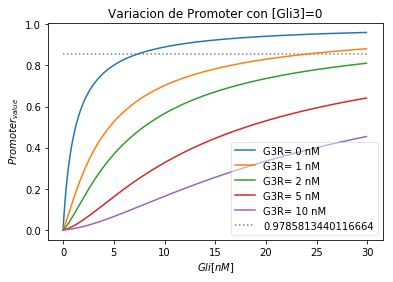
\includegraphics[width=0.8\textwidth]{variacion_promoter}
 	\centering
 	\caption{Variacion del Operador Promoter bajo la variacion de Gli3R }
 	\label{varipro}
 \end{figure}

\begin{figure}[h]
	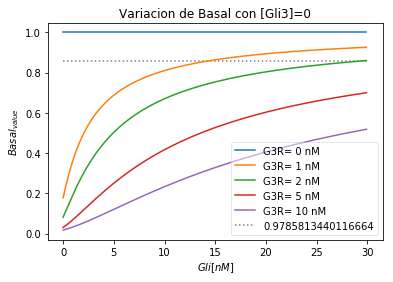
\includegraphics[width=0.8\textwidth]{variacion_basal}
	\centering
	\caption{Variacion del Operador Basal bajo la variación de Gli3R }
	\label{varibas}
\end{figure}

\subsubsection{Reducción de la complejidad del operador}

En los siguientes apartados tendremos que hacer grandes volumenes de cuentas para estudiar variaciones en el comportemiento cualitativo del modelo. Por este motivo cualquier simplificación u optimización es altemente bienvenida a la hora de programar. 

En nuestro caso, basándonos en los resultados de \cite{multiple} tuvimos acceso a una simplificación de los operadores promoter y basal. Antes de realizar el estudio, sin embargo, quisimos comprobar numéricamente la viabilidad frente a multiples variaciones de las dos expresiones. 

Prueba de ello es la figura \ref{compara}, donde mostramos como ambas expresiones son equivalentes cualesquiera variaciones hagamos. Dentro de esta tenemos en color la expresión clásica de los operadores y en líneas discontinuas mostramos la nueva expresion. Como se ve, la coincidencia es perfecta. 

\begin{figure}[h]
	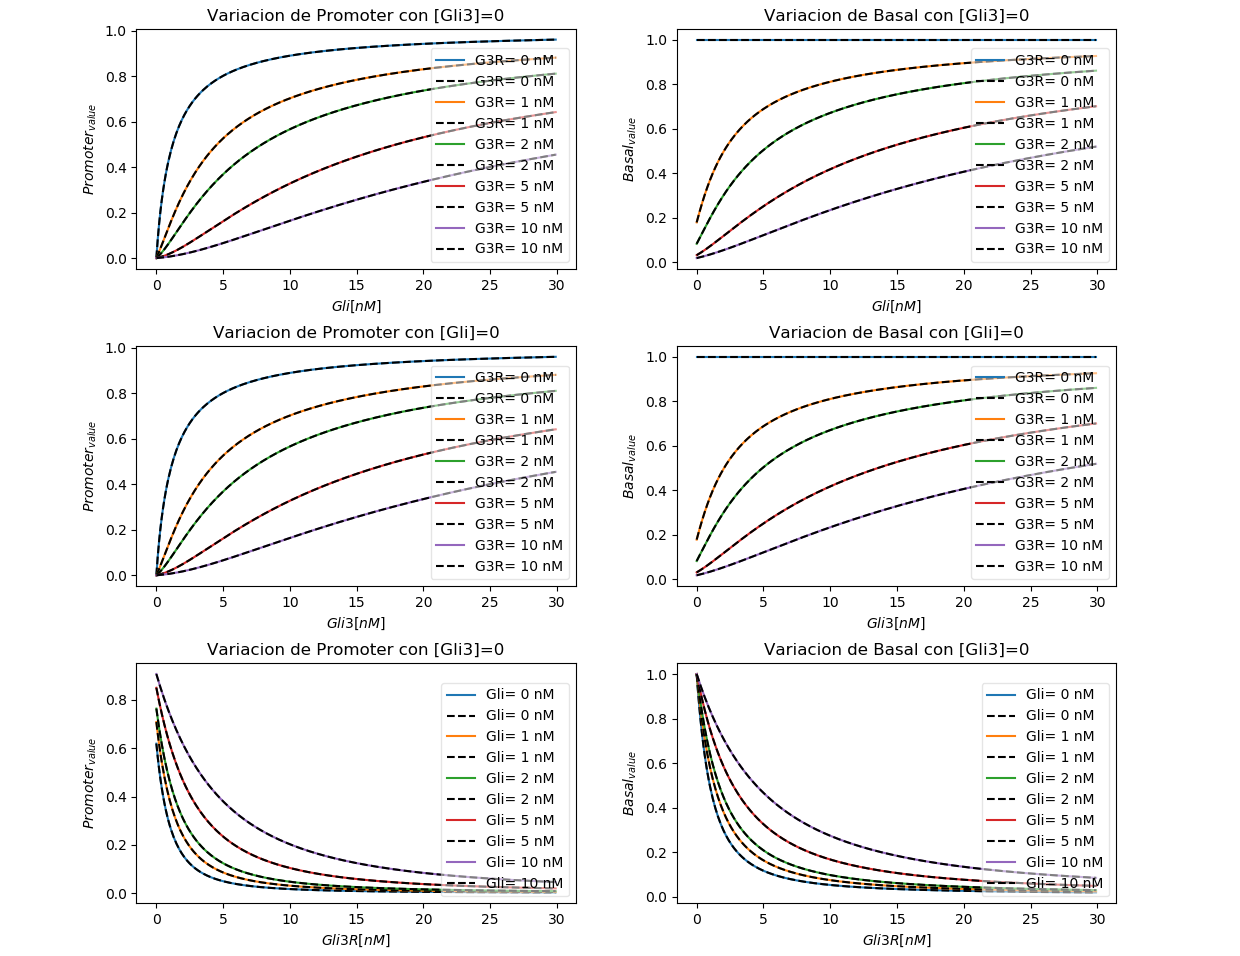
\includegraphics[width=0.8\textwidth]{reduced_form_promoter}
	\centering
	\caption{Comparación numérica de las formas de reducidas de Promoter y Basal (en negro discontinuo) frente a las formas de \cite{schaffer} }
	\label{compara}
\end{figure}

\subsection{Evolución temporal}
Una vez computamos los operadores en su forma reducida, procedimos a simular la evolución temporal del sistema. 

Para ello utilizamos el módulo de calculo numérico de Python y el algoritmo lsode que es robusto frente a comportamientos stiff. (Estos calculos ademas han sido validados y reproducidos con Octave)

En particular corrimos simulaciones con distintas condiciones iniciales y distintos valores de Shh:

\begin{itemize}
	\item lista de las condiciones (4)
\end{itemize}

Dentro de estas simulaciones preliminares, en cuanto al estudio cualitativo, observamos dos interesantes comportamientos según varía la cantidad de $Shh/k_{Shh}=0.1$ en \ref{lai1}, $Shh/k_{Shh}=1.5$ en \ref{lai2}. Esto nos confirma la multiestabilidad del sistema que se afirma en el articulo original. Pero, como veremos más adelante, esta debe ser tomada con precaución.

Los estados estacionarios sirvieron tambien de punto de partida para nuevas simulaciones, sin embargo, hay resultados de \cite{schaffer} que hemos concluido irreproducibles , destacando la dinámica del sistema con un cambio brusco de la cantidad de Shh\footnote{Figura 2(A) de \cite{schaffer}.}. 



 \begin{figure}[h]
 	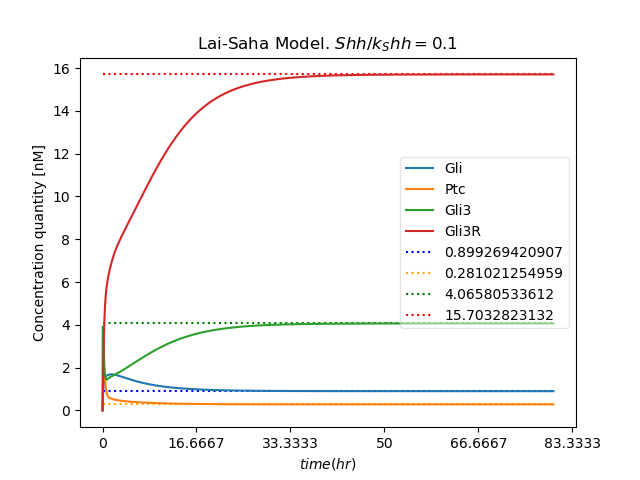
\includegraphics[width=0.8\textwidth]{lai2}
 	\centering
 	\caption{Evolución del modelo \cite{schaffer} con $Shh/k_{Shh}=0.1$ }
 	\label{lai1}
 \end{figure}


\begin{figure}[h]
	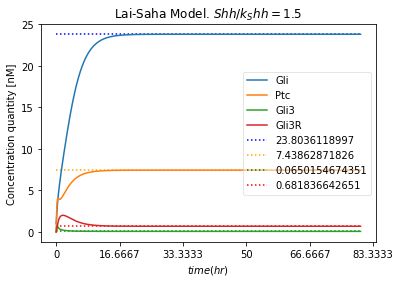
\includegraphics[width=0.8\textwidth]{lai1}
	\centering
	\caption{Evolución del modelo \cite{schaffer} con $Shh/k_{Shh}=1.5$}
	\label{lai2}
\end{figure}

\subsection{Análisis numérico de los estados estacionarios}

Para el análisis numérico de los estados estacionarios seguimos dos estrategias. 
En primer lugar programamos las expresiones analíticas obtenidas en el apartado \ref{apartado2.4}. Con ellas podemos representar la funcion y la recta $y=Gli$. 

Esta representación nos permite observar los puntos de corte de ambas funciones y, con ello inferir los estados estacionarios. Más aun, nos permite observar el comportamiento de la curva más claramente según varían los parámetros para decidir como alterarlos de manera que se produzcan puntos de corte (lo que nos dió una primera intuición sobre $r_{g3b}$).

(insertar foto de los dos progrmas)

Con esta primera parte, para analizar grandes volumenes de variaciones de parametros cambiamos el enfoque. Dado que calculamos de forma discreta, escribimos un programa que computaba la resta de ambas funciones y nos devuelve el numero de veces que la resta cambia de signo (es decir, el punto i-esimo es mayor que cero y el i-esimo +1 es menor, o vicecersa).

(isertar extracto del log que localiza los ceros en Shh y$r_{g3b}$).

Con ello, obtivumos intuicion sobre que diagramas de bifurcación computar, y obtuvimos el codigo base para explorar el nuevo modelo.



\subsection{Diagramas de bifurcación}
Durante el estudio de este modelo procedimos tambien a realizar diagramas de bifurcación\footnote{Un diagrama de bifurcación de un sistema dinámico es una estratificación de su espacio de parámetros inducida por la equivalencia topológica, junto con los retratos de fase representativos de cada estrato.} con aquellos parámetros que el análisis numérico nos mostró como relevantes. Además, procedimos a evaluar la reproducibilidad del artículo en los diagramas que presentan. 

La herramienta escogida para tal fin  fue AUTO, un motor para el cálculo de diagrama de bifurcaciones. En particular utilizamos XppAut, un interprete de AUTO que nos permite realizar continuacion, cambios de ramas y diagramas de bifurcación completos, así como el cálculo de la estabilidad de los puntos fijos. 

Para una mayor profundización en el analisis numérico de bifurcaciones puede consultarse \cite{meijer2012numerical}. Además, en mi trabajo de fin de grado \cite{Yo} puede encontrarse una guía básica de AUTO para interpretar los resultados que imprime por pantalla (se maneja desde la terminal) y como pasarlos a un diagrama. 


\subsubsection{Bifurcación bajo $Shh/K_{Shh}$}

\textbf{falta añadir la imagen del diagrama}

Debido a las diferencias que pudimos encontrar durante el desarrollo del modelo, nos pareció interesante intentar reproducir el comportamiento de Gli frente a la variación de $Shh/K_{Shh}$.  En la figura \ref{111} se puede encontrar el diagrama hallado.

En este caso, frente a los resultados del paper, obtenemos un comportamiento de interruptor bi estable, sin embargo este no es reversible si no irreversible. 

Estos resultados, aunque muestran una dinámica similar, difieren cualitativamente de \cite{schaffer}. Sin embargo una revisión bibliográfica nos mostró como se relacionan con los posteriores trabajos del equipo, en concreto \cite{saha}.




\subsubsection{Bifurcación bajo $r_{g3b}$}
Durante el desarrollo de los estados estacionarios, pudimos observar como las variciones en la tasa de sintetizacion basal del gli3 afectaban dramáticamente a los puntos de corte.

 Con ello, teniendo como referencia los códigos del apartado \ref{b} desarrollamos el diagrama de bifurcaciones de Gli frente al a variación de este parámetro \ref{lai_2}, algo que no tenemos constancia de que se hubiese llevado a cabo.

 En general, concluimos que la tasa de generacion de Gli3 juega un papel fundamental en la dinámica de este modelo, tanto por su posible alteración escogiendo como elemento delimitante Gli o Ptc como por por la variación de este en si misma. 
 
\begin{figure}[h]
	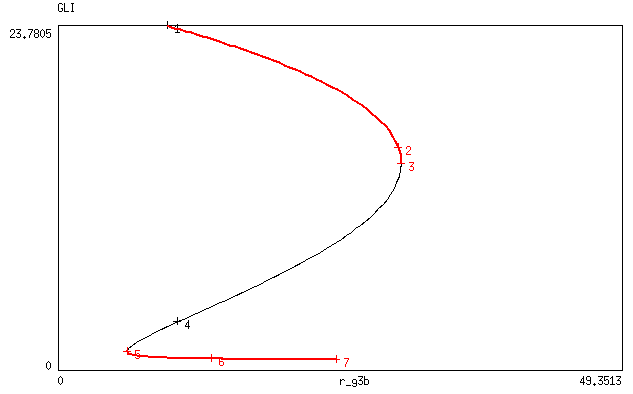
\includegraphics[width=0.8\textwidth]{gliVSr_g3b}
	\centering
	\caption{Diagrama de Bifurcación de \cite{schaffer} con $Gli$ frente a $r_{g3b}$}
	\label{lai_2}
\end{figure}

\section{Críticas}
Aun que el modelo es un referente desde hace muchos años, hemos encontrado dificultades a la hora de estudiarlo. Exponemos una breve crítica al mismo de carácter constructivo.
\begin{itemize}
	\item Posibles erratas: Si bien el comportamiento es el esperado y descrito en la mayoría de los casos, ha sido habitual durante la investigación encontrarnos con problemas a la hora de reproducir los resultados que vienen descritos en el articulo. 
	La ausencia de datos abiertos para esta tarea, la ausencia del código usado en muchos casos y, de código privativo en otros, dificulta en gran medida el estudio y reproducción. Dejamos patente que hay gráficas (corregidas en otros artículos) y expresiones con algunas erratas que pueden llevar a error.
	
	\item Algunas simplificaciones del modelo necesarias para el desarrollo del mismo pueden ser atacadas para estudiarlo en más profundidad. En particular, es nuestro enfoque añadir detalles que este modelo no contempla con el fin de estudiar si así podemos comprender mejor este proceso. 
\end{itemize}




\chapter{Modelo alternativo}

\label{ch:modelo_alternativo}

\section{Introducción}

\section{Modelado BEWARE}

\section{Sistema final}

La mayoría de cuentas del apartado se han generado con la ayuda de \cite{sympy}.

\begin{equation}
\frac{dGli}{dt} = BEWARE(Gli, Gli_3, Gli3R)-k_{deg}Gli,
\label{eq:1}
\end{equation}

\begin{equation}
\frac{dGli_3}{dt} = \frac{r_{g3b}}{Ptc}-Gli_3\left(k_{deg}+\frac{k_{g3rc}}{K_{g3rc}+Signal}\right),
\label{eq:2}
\end{equation}

\begin{equation}
\frac{dGli3R}{dt}= Gli_3\left(\frac{k_{g3rc}}{K_{g3rc}+Signal}\right)-k_{deg}Gli3R,
\label{eq:3}
\end{equation}

\begin{equation}
\frac{dPtc}{dt} = BEWARE(Gli, Gli_3, Gli3R)-k_{degp}Ptc.
\label{eq:4}
\end{equation}


Donde tenemos, por definición:
 \begin{equation}
Signal=\frac{\frac{Shh}{k_{shh}} + 1}{\frac{Shh}{k_{shh}} + 1 + \frac{Ptc}{k_{ptc}}},
\label{signal} \end{equation}

y,


\begin{equation}
BEWARE(Gli, Gli_3, Gli3R)=\frac{c_{b}}{1 + \frac{k_{RNAP}}{F_{reg}(Gli, Gli_3, Gli3R) RNAP}},
\end{equation}

donde solo nos queda describir $F_{reg}$. En el caso de de gradientes opuestos y no/total cooperatividad de los factores de transcripción nos queda:

\begin{equation}
F_{reg}=\frac{1 + \frac{1}{c} \left(\frac{Gli a_{Gli}}{k_{Gli}} c + \frac{Gli_{3} a_{Gli3}}{k_{Gli3R}} c + \frac{Gli3R c}{k_{Gli3R}} r_{Gli3R} + 1\right)^{3} - \frac{1}{c}}{1 + \frac{1}{c} \left(\frac{Gli c}{k_{Gli}} + \frac{Gli_{3} c}{k_{Gli3R}} + \frac{Gli3R c}{k_{Gli3R}} + 1\right)^{3} - \frac{1}{c}}
\end{equation}






Podemos desarrollar las funciones en cada uno de los términos, quedándonos las siguientes expresiones:
\begin{equation}
\frac{dGli}{dt}=- Gli k_{deg} + \frac{c_{b}}{1 + \frac{k_{RNAP} \left(1 + \frac{1}{c} \left(\frac{Gli c}{k_{Gli}} + \frac{Gli_{3} c}{k_{Gli3R}} + \frac{Gli3R c}{k_{Gli3R}} + 1\right)^{3} - \frac{1}{c}\right)}{RNAP \left(1 + \frac{1}{c} \left(\frac{Gli a_{Gli}}{k_{Gli}} c + \frac{Gli_{3} a_{Gli3}}{k_{Gli3R}} c + \frac{Gli3R c}{k_{Gli3R}} r_{Gli3R} + 1\right)^{3} - \frac{1}{c}\right)}}.
\end{equation}


\begin{equation}
\frac{dGli_3}{dt}=- Gli_{3} \left(k_{deg} + \frac{k_{g3rc}}{K_{g3rc} + \frac{\frac{Shh}{k_{shh}} + 1}{\frac{Shh}{k_{shh}} + 1 + \frac{ptc}{k_{ptc}}}}\right) + \frac{r_{g3b}}{ptc}.
\end{equation}

\begin{equation}
\frac{dGli3R}{dt}=Gli_{3} \left(- Gli3R k_{deg} + \frac{k_{g3rc}}{K_{g3rc} + \frac{\frac{Shh}{k_{shh}} + 1}{\frac{Shh}{k_{shh}} + 1 + \frac{ptc}{k_{ptc}}}}\right).
\end{equation}

\begin{equation}
\frac{dPtc}{dt}=\frac{c_{b}}{1 + \frac{k_{RNAP} \left(1 + \frac{1}{c} \left(\frac{Gli c}{k_{Gli}} + \frac{Gli_{3} c}{k_{Gli3R}} + \frac{Gli3R c}{k_{Gli3R}} + 1\right)^{3} - \frac{1}{c}\right)}{RNAP \left(1 + \frac{1}{c} \left(\frac{Gli a_{Gli}}{k_{Gli}} c + \frac{Gli_{3} a_{Gli3}}{k_{Gli3R}} c + \frac{Gli3R c}{k_{Gli3R}} r_{Gli3R} + 1\right)^{3} - \frac{1}{c}\right)}} - k_{deg p} Ptc.
\end{equation}




\section{Estados estacionarios}
Siguiendo con el estudio estandar que se lleva a cabo en los modelos matemáticos procedemos con un estudio sobre los estados estacionarios que podemos encontrar en nuestro modelo.

Frente a los modelos poropuestos anteriormente en \cite{saha,schaffer} nos interesa la posibilidad de no encontrar un interruptor biestable en el comportamiento cualitativo de nuestro modelo. En primer lougar procedemos aforntando el problema desde una perspectiva analítica. 

Sean las ecuaciones \ref{eq:1}\ref{eq:2}\ref{eq:3}\ref{eq:4}, si suponemos que éstas se encuentran en un estado estacionario entonces sus cantidades son constantes. Esto implica que su derivada temporal es igual a cero.

Dado que las ecuaciones continen términos complejos, nos interesamos por agruparlas, de manera que los cálculos no sean más sencillo en un primer intento de extraer información:

Por un lado de \ref{eq:1} y \ref{eq:4}:

$$\begin{cases} 0 = BEWARE(Gli, Gli_3, Gli3R)-k_{deg}Gli, \\0= BEWARE(Gli, Gli_3, Gli3R)-k_{degp}Ptc. \end{cases}$$
Si igualamos ambas ecuaciones nos queda:
\begin{equation}
 k_{deg}Gli=k_{degp}Ptc \implies \frac{k_{deg}}{k_{degp}}Gli=Ptc
\end{equation}

Por otra parte, de \ref{eq:2} y \ref{eq:3}:



$$\begin{cases} 0 = \frac{r_{g3b}}{Ptc}-Gli_3\left(k_{deg}+\frac{k_{g3rc}}{K_{g3rc}+Signal}\right), \\0=Gli_3\left(\frac{k_{g3rc}}{K_{g3rc}+Signal}\right)-k_{deg}Gli3R. \end{cases}$$

Sumando, obtenemos:

\begin{equation}
\begin{split}
0=\frac{r_{g3b}}{Ptc}-Gli_3k_{deg}-k_{deg}Gli3R & \implies \frac{r_{g3b}}{Ptc}=Gli_3k_{deg}+k_{deg}Gli3R\implies
 \\
& \implies \frac{r_{g3b}}{Gli_3k_{deg}+k_{deg}Gli3R}=Ptc
\end{split}
\end{equation}

Con estas cuentas, podemos obtener una función de $Signal$\ref{signal} modificada, la llamaremos $Signal_{modificada}$:
 \begin{equation}
 Signal_{modificada}=\frac{\frac{Shh}{k_{shh}} + 1}{\frac{Shh}{k_{shh}} + 1 + \frac{r_{g3b}}{k_{ptc}(Gli_3k_{deg}+k_{deg}Gli3R)}}.
 \end{equation}
 
Ahora, sustituimos los valores que tenemos para intentar hallar los estados estacionarios. Haciéndolo, \ref{eq:2} nos quedaría:

\begin{equation}
0 = Gli_3k_{deg}+k_{deg}Gli3R-Gli_3\left(k_{deg}+\frac{k_{g3rc}}{K_{g3rc}+Signal_{modificado}}\right),
\label{eq:2-modified}
\end{equation}
y \ref{eq:3}:

\begin{equation}
0=Gli_3\left(\frac{k_{g3rc}}{K_{g3rc}}+Signal_{modificada}\right)-k_{deg}Gli3R.
	\label{eq:3-modified}
\end{equation}

Esto nos deja un sistema de dos ecucaciones con dos incógnitas que resolvemos:




\section{Simulaciones}

\subsection{Variación del operador BEWARE}

\begin{figure}[h]
	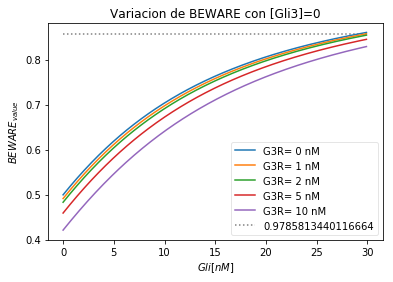
\includegraphics[width=0.8\textwidth]{variacion_new_beware}
	\centering
	\caption{Variación del nuevo operador BEWARE }
	\label{vari_beware}
\end{figure}

\begin{figure}[h]
	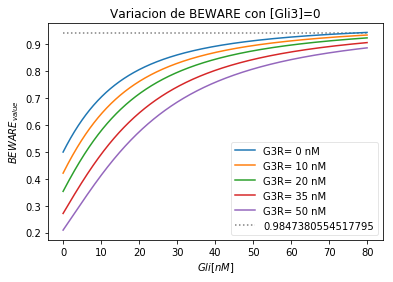
\includegraphics[width=0.8\textwidth]{variacion_new_beware_2}
	\centering
	\caption{Variación del nuevo operador BEWARE en más rango}
	\label{vari_beware_2}
\end{figure}

\subsection{Evolución temporal}

\begin{figure}[h]
	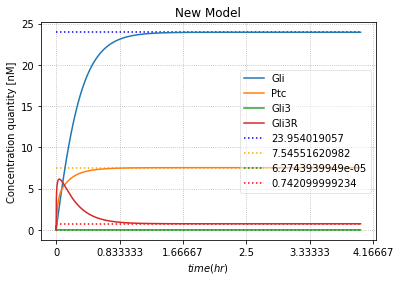
\includegraphics[width=0.8\textwidth]{new_beware_global}
	\centering
	\caption{Evolución temporal del nuevo operador BEWARE}
	\label{evolu_beware}
\end{figure}

\subsection{Análisis numérico de los estados estacionarios}




\chapter{Conclusiones}

\label{ch:conclusions}

\section{Conclusiones y trabajo futuro}
\begin{enumerate}
	\item Hemos presentado en nuestro trabajo un estudio de dos modelos utilizados para entender el sistema de señalización de Shh. 
	\item  Dentro del modelo clásico hemos observado comportamientos cualitativos y como su origen puede residir también en otros parámetros no contemplados en el artículo original.
	\item  A su vez, hemos presentado un nuevo modelado para este problema siguiendo una estrategia distinta a la original.
	\item Este modelo ha demostrado comportarse de forma parecida al original, pero con sutiles diferencia en cuanto a la estabilidad. En concreto este modelo no presenta un swicth biestable en su comportamiento. Este hecho apoya la teoría de que este modelo capta de forma correcta la realidad biológica observada en la práctica.
	\item Nos gustaría seguir desarrollando este proyecto. Si bien el numérico a demostrado ser una interesante herramienta para captar tendencias cualitativas en nuestro modelo, necesitamos una solida prueba teórica.
	\item Para ello, a parte de utilizar barridos de parámetros mayores, queremos investigar si podemos obtener una prueba teórica de este resultado. Iniciamos este trabajo con un fin teórico, sin embargo la complejidad de las operaciones resiste nuestros envites de resolución actuales. Aún así, las pruebas numéricas sostienen que vamos por buen camino.
\end{enumerate}



 

 
 
 



\addcontentsline{toc}{chapter}{Bibliografía}
\bibliographystyle{apalike}
\bibliography{bibliography/bibliografia}

\appendix
\chapter{Códigos}
\label{ch:app}
Los códigos también se pueden consultar en \url{https://github.com/thebooort/shh-signal-model}
\section{Python}

Variabilidad del nuevo operador BEWARE

\lstinputlisting[language=Python]{scripts/python_codes/beware_variability.py}

Variabilidad de los operadores promoter y basal de \cite{saha}.

\lstinputlisting[language=Python]{scripts/python_codes/promoter_basal_variability.py}

Comparativa entre las expresiones de BEWARE.

\lstinputlisting[language=Python]{scripts/python_codes/comparativa_script.py}

Script para contar los ceros.

\lstinputlisting[language=Python]{scripts/python_codes/counting_zeros.py}

Definición y simulación del sistema con el nuevo operador BEWARE.

\lstinputlisting[language=Python]{scripts/python_codes/definition_script.py}

Scrip para representar la ecuacion de punto fijo.

\lstinputlisting[language=Python]{scripts/python_codes/fixed_points.py}

Definición y simulación del sistema con el operador BEWARE de \cite{saha}.

\lstinputlisting[language=Python]{scripts/python_codes/lai_saha_model.py}

Script para localizar los ceros por las veces que la resta de dos expresiones corta el eje de abcisas.

\lstinputlisting[language=Python]{scripts/python_codes/locating_zeros.py}

Cáculo simbólico.

\lstinputlisting[language=Python]{scripts/python_codes/steady_states_symbolic.py}
\section{Octave}

Operador BEWARE en Octave.

\lstinputlisting[language=Octave]{scripts/octave_codes/f.m}

Script para simular el sistema.

\lstinputlisting[language=Octave]{scripts/octave_codes/simulation.m}
\section{XppAut}
Script tipo \textit{.ode} para simular los diagramas de bifurcación con el nuevo BEWARE.

\lstinputlisting[language=C]{scripts/xppaut_codes/beware_model.ode}

Script tipo \textit{.ode} para simular los diagramas de bifurcación con el BEWARE clásico.

\lstinputlisting[language=C]{scripts/xppaut_codes/lai_saha.ode}


\end{document}
